\chapter{Proof of concept}
\label{ch:proof-of-concept}



In dit hoofdstuk werd getracht om, steunend op een proof of concept, een antwoord te bieden op de laatste deelvraag van het onderzoek:

\begin{center}
	\textit{\textbf{``Hoe kunnen softwareontwikkelaars de data van hun ERP-systeem opslaan in een blockchain?''}}
\end{center}

Het opzet van deze proof of concept, was in eerste instantie om aan te tonen dat het effectief gelukt is om data op te slaan in een blockchain. Hiervoor werd gebruik gemaakt van de services van mintBlue. Daarenboven wordt met deze proof of concept ook de aanzet gegeven tot een echte use case voor dit gegeven: NFT invoicing. Tot slot wordt ook een schets gemaakt van het kostenplaatje dat hierbij komt kijken. Het hoofdstuk eindigt met een kritische noot.


\section{Data op de blockchain plaatsen}
\label{sec:data-op-de-blockchain-plaatsen}

Zoals al vermeld in Sectie \ref{sec:nfts} -- \nameref{sec:nfts} is het mogelijk om eender welke data op te nemen in een blockchain. In deze sectie staat beschreven hoe data uit het ERP-systeem op de blockchain geplaatst kan worden. Meer bepaald de data van een digitale factuur.

\subsection{Digitale facturen}
\label{sub:digitale-facturen}

Zoals kort aangehaald in Sectie \ref{sec:enterprise-resource-planning} -- \nameref{sec:enterprise-resource-planning} zijn er verschillende manieren om facturen digitaal op te slaan en uit te wisselen.
Bij voorkeur wordt hiervoor een bestand gebruikt dat de data van die factuur op een gestructureerde manier bijhoudt. Dergelijke bestanden worden ook wel e-invoices genoemd. Hiervoor bestaan een aantal gangbare formaten zoals EDI, XML of CSV~\autocite{Damsgaard2000}. Als bestuurslid van werkgroep UBL.BE\footnote{UBL.BE werd opgericht met als doel het gebruik van elektronische documenten in kmo's te bevorderen. De vereniging zet in op UBL-standaarden om uitwisseling van documenten tussen ondernemingen te vergemakkelijken.}, maakt 14IT gebruik van XML-bestanden. Deze worden opgebouwd volgens syntax en regels die werden vastgelegd in de UBL-standaard. Daarom noemt men dit ook, kortweg, UBL-bestanden. Onder die vorm, is een e-invoice in se een tekstbestand waarin factuurgegevens genoteerd staan aan de hand van vastgelegde XML-tags. Het adres van de klant zou hierin bijvoorbeeld als volgt kunnen voorkomen:

\begin{figure}[H]
	\centering
	\includegraphics[width=\linewidth]{img/proof-of-concept/xml-example.pdf}
\end{figure}


\subsection{Data wegschrijven}
\label{sub:data-wegschrijven}

Aangezien digitale facturen niet meer zijn dan een gestructureerd XML-bestand, kunnen ze als NFT gemint worden. Dat betekent dat er een ``transactie'' met (verwijzing naar) de factuur op de blockchain geplaatst kan worden. Om dit principe aan te tonen, werd --in het licht van dit onderzoek-- een mock-factuur opgesteld. Het bestand werd in \href{https://whatsonchain.com/tx/71054b6b9aef47124cc5db9983a06d7608ec408c1ed3ee3a0ad0e34e2951c83c}{\textcolor{blue}{transactie 710...83c}} op de BSV-blockchain gebracht. Figuur~\ref{fig:factuur-transactie} geeft de inhoud van de transactie weer, zoals deze te vinden is via een online \textit{block explorer}. Volgende paragrafen geven meer uitleg bij de details van deze transactie.

Op blok \#738410 van de BSV-blockchain bevindt zich een transactie die de mock-factuur van deze bachelorproef bevat. Een transactie is en blijft nog steeds een bitcoin-uitwisseling van input naar output. De bitcoin (in dit geval BSV) kunnen over meerdere outputs verdeeld worden. Het is zelfs mogelijk om outputs van 0 BSV op te nemen. Hier wordt handig gebruik van gemaakt om de data van de factuur op te slaan.

In ons voorbeeld werd een input van 0.00001968 BSV ``verdeeld'' over twee outputs. Om miners aan te moedigen deze transactie op te nemen in het blok, werd een \textit{fee} betaald van 0.00000303 BSV. Het overblijvende bedrag gaat integraal naar output \#1. Dit stelt een uitwisseling voor van 0.00001665 BSV van en naar hetzelfde adres 1AT...uyy.

Output \#0 is een \textit{data-carrying} output. Het werd uitsluitend gecreëerd als vehicel voor de data van de factuur. Daarom gaat er 0 BSV naartoe en kent het tevens geen adres. De \verb|OP_RETURN| geeft aan dat dit over een output gaat die niet gespendeerd kan worden. In het bijhorende tekstveld zien we de voornaamste inhoud van deze output, namelijk de digitale factuur.

\begin{figure}[H]
	\centering
	\includegraphics[width=\linewidth]{img/proof-of-concept/factuur-transactie.png}
	\caption{\label{fig:factuur-transactie}E-invoice als transactie op de BSV-blockchain}
\end{figure}

De e-invoice is vanaf nu dus definitief aanwezig als data op de BSV-blockchain. Kortom betekent dit dat de factuur digitaal beschikbaar is voor de ontvanger. Elke BSV-node kan ze opvragen via het \verb*|TXID| van de omvattende transactie. Het is echter geen vereiste om een eigen node op te zetten. Publieke API's zoals die van Blockchair maken het mogelijk om met een eenvoudige \href{https://api.blockchair.com/bitcoin-sv/raw/transaction/031fcc00b88fcc2252107be98c085eea528c470df9d910387947f60adae80287}{\textcolor{blue}{URL}} de ruwe data (JSON) van een transactie op te vragen. De factuur kan uitgelezen worden door de \verb*|hex|-waarde van \verb*|vout| \verb*|0| om te zetten naar ASCI. De \textit{block explorer} in Figuur~\ref{fig:factuur-transactie} doet dit automatisch.


\begin{figure}[H]
	\centering
	\includegraphics[width=0.8\linewidth]{img/proof-of-concept/ruwe-transactie.png}
	\caption{\label{fig:ruwe-transactie}Ruwe data van de transactie}
\end{figure}

\subsection{Encryptie}
\label{sub:encryptie}

Voorgaande subsectie toont aan dat het mogelijk is om de data van een digitale factuur op te slaan in een blockchain. Aangezien BSV een publieke blockchain is, is die factuur ook publiekelijk toegankelijk.

In plaats van de factuur rechtstreeks op de blockchain te plaatsen, zou het er ook geëncrypteerd opgeplaatst kunnen worden. Enkel partijen die beschikken over de \textit{encryption secret} zullen de data kunnen decrypteren en zo de factuur inkijken. 

\begin{figure}[H]
	\centering
	\includegraphics[width=\linewidth]{img/proof-of-concept/transactie-encryptie.png}
	\caption{\label{fig:transactie-encryptie}Transactie met geëncrypteerde e-invoice}
\end{figure}


\section{NFT invoicing}
\label{nft-invoicing}

Voorgaande sectie toont aan dat het mogelijk is om data uit het ERP-syteem op te slaan in een blockchain. De nodige encryptie zorgt ervoor dat enkel de bestemde partij ook toegang krijgt tot die data. Dit gegeven schept nieuwe mogelijkheden binnen het hele EDI-gebeuren.

\subsection{EDI-proces}
\label{sub:edi-proces}

Om de geëncrypteerde factuur uit Subsectie \ref{sub:encryptie} -- \nameref{sub:encryptie} uit te lezen, dient men de juiste transactie op te halen en vervolgens de \textit{data-carrying} output te decrypteren. Dit proces kan geprogrammeerd worden en afgeschermd als zijnde een API-methode. Deze vormt een endpoint die in het geval van een REST API zelfs met een URL kan aangesproken worden. De ontvanger kan de \verb|TXID| in combinatie met de \textit{encryption secret} dan gebruiken als token voor de digitale factuur.

Bovenstaand gegeven kan voor CPSolution concreet gebruikt worden voor een nieuw EDI-proces genaamd NFT invoicing.

Wanneer bedrijf A een factuur opstelt in CPSolution, wordt de bijhorende data opgeslagen in de SQL Server databank. Met behulp van een webservice wordt de factuur geëxtraheerd als UBL-bestand. Dit bestand wordt vervolgens geëncrypteerd op de blockchain geplaatst. Zo bekomt men een transactie zoals die in Figuur~\ref{fig:transactie-encryptie}. 

De factuur is vanaf dat moment immutable en staat klaar om opgehaald te worden. Ophalen kan --zoals hierboven reeds aangehaald-- met een API-methode die op basis van de \verb|TXID| en \textit{encryption secret} de juiste transactie ophaalt en decrypteert. Vervolgens dient men, op basis van de \verb|TXID| en \textit{encryption secret} de juiste URL op te stellen om deze methode op te roepen. Deze URL kan op zijn beurt aangeboden worden onder de vorm van een QR-code. Het downloaden van de factuur herleidt zich dan tot het simpelweg scannen van deze code. Figuur~\ref{fig:qr-code} kan gescand worden om de mock-factuur uit Sectie \ref{sub:digitale-facturen} -- \nameref{sub:digitale-facturen} op te halen.

\begin{figure}[H]
	\centering
	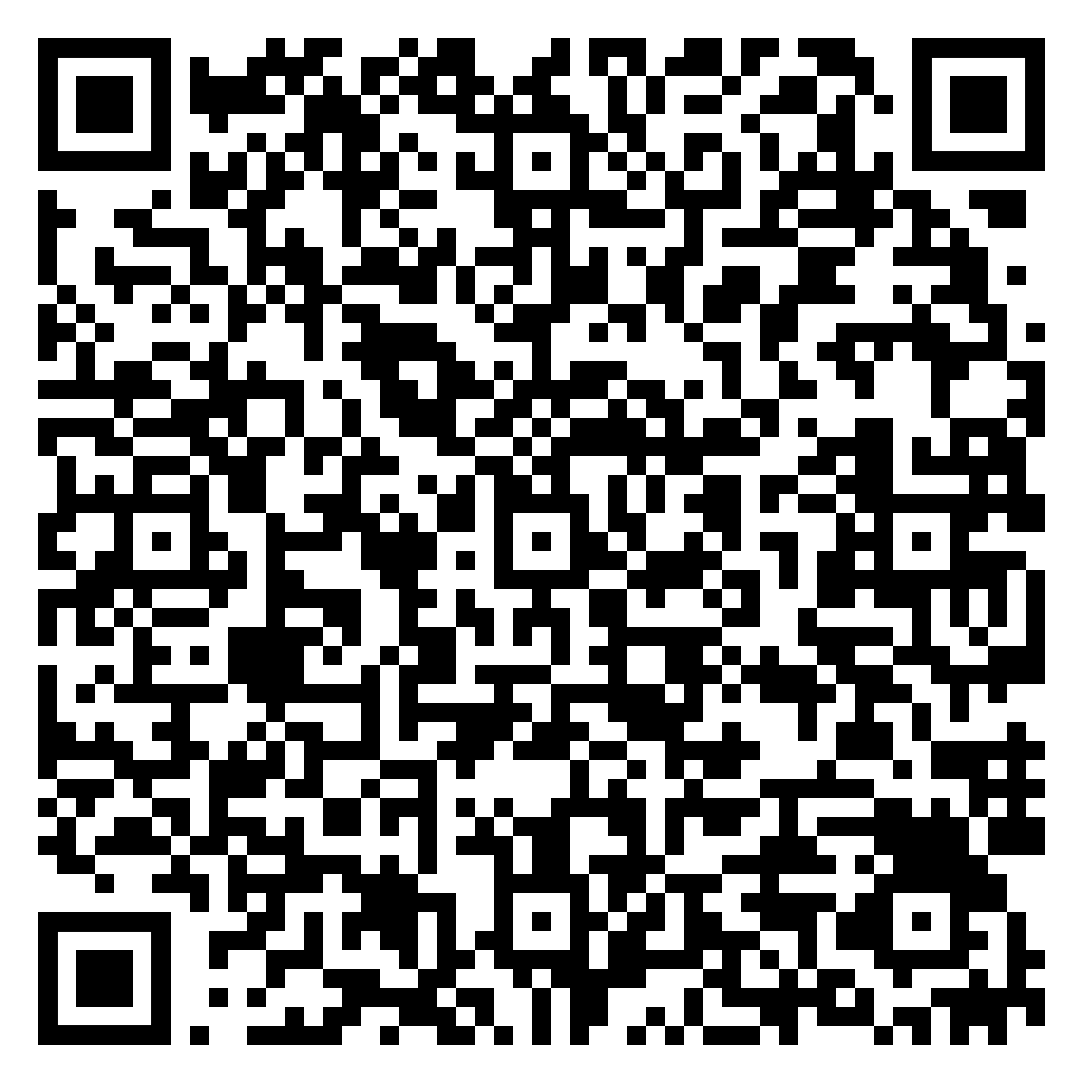
\includegraphics[width=0.25\linewidth]{img/proof-of-concept/qr-code.pdf}
	\caption{\label{fig:qr-code}QR-code om e-invoice op te halen van de BSV-blockchain}
\end{figure}

Op hetzelfde moment genereert CPSolution een pdf voor de fysieke factuur. Bijlage \ref{ch:mock-factuur} -- \nameref{ch:mock-factuur} is een voorbeeld van hoe deze papieren variant er zou kunnen uitzien. De QR-code wordt op dit fysieke document geplaatst. Daarmee bevat deze een verwijzing naar de bijhorende e-invoice, zoals die op de blockchain staat.

\begin{figure}[H]
	\centering
	\includegraphics[]{img/proof-of-concept/nft-invoicing.pdf}
	\caption{\label{fig:nft-invoicing}NFT invoicing}
\end{figure}

Bedrijf A zendt vervolgens deze fysieke factuur uit naar bedrijf B\footnote{Briefverkeer is vandaag de dag nog steeds een vaste waarde in het bedrijfsleven.}. Wanneer het personeel uit bedrijf B het document goedkeurt, kunnen ze de QR-code scannen. De e-invoice wordt automatisch gedownload en kan worden opgenomen in het eigen ERP-systeem of boekhoudpakket. 

\subsection{Voordelen}
\label{sub:voordelen}

NFT invoicing biedt als voordeel dat er steeds een referentie beschikbaar blijft naar de originele digitale versie van een factuur. Aangezien die versie op de blockchain staat, weet de ontvanger zeker dat deze ongewijzigd is. Het gedistribueerde en onvervalsbare karakter van de \textit{ledger} maken een ``\textit{single source of truth}'' mogelijk tussen meerdere onderhandelende partijen. Dit was een doel dat voorheen enkel nagestreefd werd binnen eenzelfde ERP-systeem\footnote{Zie Sectie \ref{sec:enterprise-resource-planning} -- \nameref{sec:enterprise-resource-planning}}. De immutability en transparantie van de blockchain zouden tevens allehande fraude zoals spookfacturen kunnen helpen tegengaan~\autocite{Sterk2021}. 

Anderzijds kan er met NFT-invoicing nog steeds voldaan worden aan de voorkeur van veel bedrijven om met fysieke documenten te werken. Om die papieren facturen op te nemen in het boekhoudsysteem, worden nu vaak OCR-technieken gebruikt. Dat is niet altijd evident aangezien de structuur van elk type factuur anders kan zijn. Daardoor moet de data telkens op een andere manier geïnterpreteerd worden door het boekhoudpakket. Door met een QR-code te werken, kan men vlot de originele digitale factuur ophalen. Deze kan veel vlotter ``overgegoten'' worden in een digitaal systeem aangezien het opgebouwd is volgens de UBL-standaard. Er moet dus maar een vertaling van UBL naar het eigen systeem voorzien worden, in plaats van een aparte vertaling voor elk type factuur.

\section{mintBlue}
\label{sec:mintBlue}

Softwarebedrijf mintBlue beweert het eerste publieke blockchain platform van Europa aan te bieden dat op grote schaal gebruikt kan worden. Het bedrijf, met vestigingen in Amsterdam en Antwerpen, ontwikkelt een API waarmee ontwikkelaars data kunnen opnemen in een blockchain. De infrastructuur steunt op de BSV-blockchain. In die zin biedt mintBlue zelf geen platform, maar wel een Blockchain PaaS. Vaak spreekt men simpelweg over Blockchain as a service. De naam ``mintBlue'' wordt uitwisselbaar gebruikt voor zowel het bedrijf als de service die ze bieden.

Het doel van mintBlue is om ontwikkelaars een gebruiksvriendelijke manier te bieden om lees- en schrijfoperaties van en naar de blockchain uit te voeren. Hiervoor bieden ze een API en SDK. Met behulp van deze service zou 14IT blockchain kunnen integreren in CPSolution, zonder eigen knopen of andere infrastructuur op te zetten of te onderhouden.

De services van mintBlue bevinden zich momenteel nog in een ontwikkelfase, waardoor ze nog niet publiekelijk beschikbaar zijn. Er is wel al een solide basis aanwezig. In het kader van deze bachelorproef werd vroegtijdige toegang tot het platform verleend.

\subsection{API}
\label{sub:api}

Met een API probeert mintBlue de complexiteit van een blockchain af te schermen. In eerste instantie voorziet deze POST- en GET-methodes voor transacties. Een ontwikkelaar kan dus snel een ``Write'' of ``Retrieve'' van een transactie naar de blockchain uitvoeren.

Daarnaast specifieert de API ook een aantal methodes om gebruik van het platform te ondersteunen, of om wisselwerking met Zapier\footnote{Zapier is een automatisatietool waarmee output van een toepassing zoals e-mail of Google Drive kan gebruikt worden als trigger voor input in bijvoorbeeld de mintBlue-integratie. Op die manier kan men bijvoorbeeld een Zapier-proces definiëren dat bij het ontvangen van specifieke mails een bijhorende transactie op de blockchain plaatst. Deze integraties werden niet gebruikt bij deze bachelorproef.} mogelijk te maken.

Een interessante deelverzameling is de Token API. Deze stelt developers in staat om volledige bestanden, zoals facturen of creditnota's, als NFT op de blockchain te plaatsen. De bestanden worden standaard geëncrypteerd, zodat ze enkel geraadpleegd kunnen worden met behulp van een referentie en secret.

Een eenvoudige manier om de API te benaderen, is met de mintBlue SDK. Voorlopig bestaat er enkel een SDK voor JavaScript. De bedoeling is dat er ook SDK's voor Elixir, Ruby en PHP ontwikkeld worden.

\subsection{Platform}
\label{sub:platform}

Het webplatform biedt een centraal dashboard om allerlei statistieken van uw account te raadplegen. Een project is een verzameling waaronder transacties op de blockchain gepubliceerd kunnen worden.

Figuur~\ref{fig:mintblue-project} is een weergave van de transacties die onder het project ``Bachelorproef'' gepubliceerd werden. Het transactie-adres kan geopend worden in een externe \textit{block explorer} om de inhoud in te kijken.
Ook de status van de transactie  wordt weergegeven. Dit geeft weer of de data al gepubliceerd is op de blockchain, of nog in afwachting is. Eens de transactie gepubliceerd is, moet ze nog geconfirmeerd worden op de blockchain. Voor elk blok dat na het transactieblok volgt, krijgt de transactie een ``confirmatie'' bij. Hoe groter dit getal is, hoe meer zekerheid erover bestaat dat de transactie effectief deel uitmaakt van ``de correcte'' \textit{ledger}.

\begin{figure}[H]
	\centering
	\includegraphics[width=\linewidth]{img/proof-of-concept/mintblue-project.png}
	\caption{\label{fig:mintblue-project}Project met transacties op het mintBlue-platform}
\end{figure}

Daarnaast biedt het platform ook een tool genaamd de ``composer''. Het is een grafische interface die helpt bij het opstellen van de juiste JSON voor een transactie. De GUI helpt om data, bestanden of scripts in te voeren. De bijhorende JSON wordt weergegeven.


\section{Kosten}
\label{sub:kosten}

Blockchains bieden op het vlak van opslagkosten een heel bijzondere manier om data te bewaren. Zoals werd opgemerkt in Subsectie \ref{sub:data-wegschrijven} -- \nameref{sub:data-wegschrijven} gaat het opslaan van data steeds gepaard met een transactie waarvoor een zekere \textit{fee} betaald moet worden. Die \textit{fee} moet miners ``aanmoedigen'' om de gepubliceerde transactie op te nemen in het volgende datablok. Eens een transactie deel uitmaakt van de blockchain, wordt het voor altijd bewaard door het collectieve netwerk. Opslaan in de blockchain gaat dus gepaard met een eenmalige kost van het publiceren, niet van het onderhoud\footnote{De kost van de infrastructuur waaruit het blockchain-netwerk is opgebouwd, wordt gedragen door de deelnemers die knopen voorzien. Deze hebben hun eigen incentive voor het draaiend houden van deze hardware, zoals het verdienen van \textit{fee}'s, aanbieden van een \textit{block explorer}, \textit{minen} van cryptomunten, ...}. 

Dit staat in contrast met andere --eerder klassieke-- vormen van dataopslag. Opties zoals een eigen databank of cloud, gaan altijd gepaard met een zekere maintenance-kost die moet betaald worden door de partij die de data wilt stockeren. 
Vaak betekent dit een periodieke betaling zoals een maandelijkse abonnementskost.

\subsection{mintBlue}
\label{sub:mintblue}

Dankzij bovenstaand gegeven rekent mintBlue af in functie van de hoeveelheid gepubliceerde data. Om iets op de blockchain te plaatsen, betaalt men eenmalig een vaste prijs per kilobyte. Die eenheidsprijs is afhankelijk van de afgesloten formule, met als bedoeling een zekere winstmarge te hebben op de benodigde \textit{fee}'s. Grotere transacties vereisen namelijk grotere \textit{fee}'s. Gelukkig (maar niet per toeval) maakt mintBlue gebruik van de BSV-blockchain, die een grote block size heeft van doorgaans 4GB\footnote{Er bestaat geen opgelegde limiet op de grootte van blokken. Op dit moment werken miners echter voornamelijk aan blokken van 4 GB.}. Daardoor zijn de \textit{fee}'s relatief klein. Voor de mock-factuur uit Subsectie \ref{sub:data-wegschrijven} -- \nameref{sub:data-wegschrijven} (van ongeveer 6000 B) bedroeg de \textit{fee} 0.00000303 BSV, wat op het moment van schrijven ongeveer \euro 0.0002 waard is. De prijs die mintBlue doorrekent aan de klant hangt af van de afgesloten formule. Tabel~\ref{tab:mintblue-pricing} geeft de huidige specificaties weer. Opmerkelijk is dat er met \textit{basic} en \textit{enterprise} toch een bijkomende abonnementskost is. Deze opties brengen wel meer support met zich mee.

\begin{table}[H]
	\centering
	\begin{tabular}{@{}lccc@{}}
		\cmidrule(l){2-4}
		& \textbf{Free}                                                & \textbf{Basic} & \textbf{Enterprise} \\ \midrule
		Fee          & \euro 0                                                          & \euro 49 per month & custom              \\ \midrule
		Price per kB & \begin{tabular}[c]{@{}c@{}}\euro 0,02\\ (1 MB free)\end{tabular} & \euro 0,01         & \euro 0,005             \\ \midrule
		Projects     & 3                                                            & 10             & unlimited           \\ \midrule
		Support & community     & e-mail         & support manager     \\ \bottomrule
	\end{tabular}
	\caption{\label{tab:mintblue-pricing}Prijzen van mintBlue}
\end{table}

Met bovenstaande tabel kan een eerste schatting gemaakt worden van de kosten die 14IT zou moeten betalen om facturen op te slaan. Om een representatief beeld te schetsen, kan uitgegaan worden van een klant die maandelijks gemiddeld 350 facturen opmaakt. Na een steekproef werd de grootte van een doorsnee UBL-factuur ingeschat op 6 kB. Zelfs met een ruime marge is het veilig om de grootte van een gemiddelde transactie af te ronden op 8 kB. Bij een dergelijke klant lijkt de ``Free''-formule de beste optie. De 2800 kB aan data die maandelijks verwerkt moet worden, zou telkens ongeveer \euro 56 kosten. De ``Basic''-formule wordt voordeliger vanaf een omvang van 4900 kB, of ongeveer 613 facturen.

\subsection{Overwegingen}
\label{sub:overwegingen}

Bovenstaande inschatting maakt duidelijk dat de services van mintBlue op het eerste gezicht duurder zijn dan de een traditionele cloud. Daarom moet ingeschat worden of de voordelen van NFT invoicing ook opwegen tegen de kosten. Hierbij kan men volgende overwegingen maken:

\begin{itemize}
	\item NFT invoicing kan aangeboden worden als bijkomende module van CPSolution en ook op die manier doorgerekend worden. Zo kan elke kmo voor zichzelf de inschatting maken of de voordelen wel opwegen tegenover de kosten. Indien voldoende klanten gebruik maken van deze module is een aangepaste ``Enterprise''-formule met mintBlue misschien wel aan de orde. Dat kan globaal genomen de kosten nog meer drukken.
	\item Eens data zich op de blockchain bevindt, blijft deze daar kosteloos en definitief aanwezig. Dat kan interessant zijn voor facturen aangezien deze volgens de wet minstens zeven jaar bijgehouden moeten worden. Bij cloud-oplossingen zou dit ook zeven jaar aan maintenance-kosten beteken. 
	\item Gezien de eenheidsprijs is een maand met weinig of geen facturen ook een maand met weinig of geen kosten. 
	\item NFT-invoicing biedt een alternatief voor de huidige EDI van CPSolution. Deze steunt op de services van Basware, wat ook gepaard gaat met een eigen kostenplaatje. In die context zijn de uitgaven aan mintblue niet bijkomend, maar vervangend.
\end{itemize}

Daarnaast is het niet meteen duidelijk welke invloed de koers van de BSV heeft op de kostprijs van mintBlue-transacties. CIO Pieter Den Dooven beweert althans dat het mogelijk is om een fixed price te blijven aanrekenen. Hiervoor werden contracten met datacenters gesloten. Daarnaast is BSV ook een blockchain zonder beperking op de \textit{block size}, waardoor transaction \textit{fee}'s niet oplopen zoals bij BTC bijvoorbeeld het geval is\autocite{MNP2021}.


\section{Kritische noot}
\label{sec:kritische-noot}

NFT invoicing heeft als opzet om een zekere vorm van onvervalsbaarheid te verkrijgen. Dat is dan ook gelukt: een onwijzigbare versie van de factuur staat definitief op de blockchain zoals de crediteur ze oorspronkelijk opmaakte. Fraudeurs kunnen echter nog op een andere manier proberen toeslaan: door de papieren factuur te onderscheppen en de QR-code te vervangen door een nieuwe QR-code die verwijst naar een eigen spookfactuur. De ontvanger zou de factuur goedkeuren op basis van de papieren versie, maar in het boekhoudsysteem zou de frauduleuze data binnensijpelen. Op die manier kan een overschrijving plaatsvinden naar de oplichter.

Een fraudeur zou hiermee echter een volledig spoor achterlaten van zijn bedrog. Een blockchain blijft in se nog steeds een keten van transacties. Bij elke transactie horen adressen die op hun beurt bij een zekere identity horen. Door het spoor aan transacties te volgen, zouden overheidsdiensten de oplichter kunnen vatten\footnote{Op die manier werden al criminelen opgespoord die de blockchain gebruikten als medium voor illegale praktijken zoals drugshandel en kindermisbruik.}~\autocite{Bohannon2016}. Hoewel het dus technisch mogelijk is om op deze manier spookfacturen uit te zenden, lijkt het er niet meteen op dat de blockchain hiervoor het geschikte medium is (vanuit de ogen van de fraudeur).

Bij mintBlue wordt in elk geval nog aan een oplossing met behulp van \textit{digital signatures} gewerkt. Hiervoor wordt een samenwerking op poten gezet met de Kamer van Koophandel. De KVK dataservice bevat alle actuele informatie uit het handelsregister. Door de publieke sleutel van elke onderneming op te nemen in de databank van de Kamer van Koophandel, wordt het voor iedereen mogelijk om te verifiëren of de digitale factuur van de juiste partij afkomstig is. Met deze samenwerking berust men echter opnieuw op een zeker vorm van authoritaire derde partij. 




